\documentclass[journal,12pt,onecolumn]{IEEEtran}
\usepackage[utf8]{inputenc}   % Codificación de entrada
\usepackage[T1]{fontenc}      % Codificación de fuente
\usepackage[spanish,es-tabla]{babel}   % Idioma español
\usepackage{lmodern}          % Fuente moderna
\usepackage{amsmath, amssymb} % Matemáticas y símbolos
\usepackage{graphicx} 		  % Gráficos e imágenes
\graphicspath{{img/}{tablas/}{portada/}}  % Las imágenes se buscarán en la carpeta "img"
\usepackage{longtable}      % Para tablas que se extienden en varias páginas
\usepackage{tabularx}	% Tablas avanzadas
\usepackage{threeparttable}
\usepackage{hyperref}	% Hipervínculos

%-------------------------------------------
% Otros paquetes útiles (personaliza según tus necesidades)
%-------------------------------------------
\usepackage{caption}
\usepackage{subcaption}
\usepackage{xcolor}
\usepackage{setspace}


%-------------------------------------------
% Comandos personalizados
\renewcommand{\listtablename}{Índice de tablas}
\renewcommand{\appendixname}{Anexos}
\definecolor{colorreferences}{RGB}{48,134,3}

% Metadatos del PDF
\hypersetup{
	unicode=true,
	hidelinks,
	colorlinks=true,       % false: boxed links; true: colored links
	linkcolor=black,          % color of internal links (change box color with linkbordercolor)
	citecolor=colorreferences,        % color of links to bibliography
	filecolor=magenta,      % color of file links
	urlcolor=blue,           % color of external links
	linkbordercolor={0 0 0}
}
%-------------------------------------------
% Inicio del documento
%-------------------------------------------
\begin{document}

% Aquí se encuentra el archivo con la portada
\begin{titlepage}
	\centering
	%-------------------------------------------
	% Logos en una tabla: izquierda, centro y derecha
	\begin{tabular}{@{}p{0.3\textwidth} p{0.3\textwidth} p{0.3\textwidth}@{}}
		
\includegraphics[height=2cm]{tecnm} & 
		\centering 
\includegraphics[height=1.5cm]{SEP} & 
		\raggedleft 
\includegraphics[height=2cm]{ith.jpg} \\
	\end{tabular}
	
	\vspace{2em}
	
	\noindent
	%-------------------------------------------
	%	Información institucional y académica (esquina superior izquierda)
	\begin{minipage}[t]{0.48\textwidth}
		\raggedright
		\small \textbf{%
			Instituto Tecnológico de Hermosillo\\
			Materia: Robótica\\
			Profesor: Medina Gil Lamadrid, Jesús Iván%
		}
	\end{minipage}%
	\hfill
	%	fecha actual (esquina superior derecha), en letras pequeñas y en negrita.
	\begin{minipage}[t]{0.48\textwidth}
		\raggedleft
		\small \textbf{\today}
	\end{minipage}
	
	\vspace{2em}
	
	%-----------------------------------------
	% Unidad y Título de la tarea en letras grandes y en negrita
	{\large \textbf{Unidad 1: Morfología del robot}}\\
	{\Huge \textbf{Tipos de Sensores}}
		
	\vspace{1em}
	
	%---------------------------------------
	% Tabla con la información del equipo
	%---------------------------------------
	% Encabezado del equipo
	\begin{center}
		{\Large \textbf{Equipo 3}}
	\end{center}
	
	\vspace{1em}
	
	% Tabla de integrantes:
	% Cada fila contiene: foto (columna izquierda) y datos del integrante (columna derecha)
	\begin{center}
		\begin{tabular}{c c}
			\begin{tabular}{c}
				
\includegraphics[height=3cm]{Miguel.jpg} \\
				\textbf{Bojorquez Pedroza},\\ Miguel Ángel \\ \texttt{l21330540@hermosillo.tecnm.mx} \\ Teléfono: 6321127584
			\end{tabular} &
			\begin{tabular}{c}
				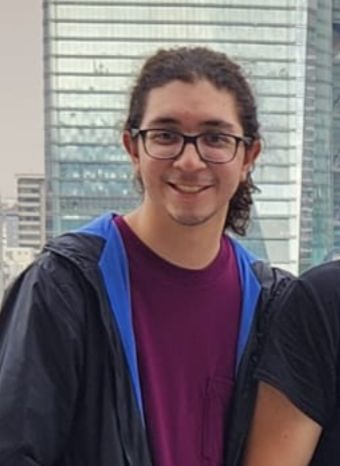
\includegraphics[height=3cm]{Bruno.jpg} \\
				\textbf{Díaz Garnica,}\\ Bruno \\ \texttt{l21330564@hermosillo.tecnm.com} \\ Teléfono: 6623951051
			\end{tabular} \\ \vspace{2em}
			\begin{tabular}{c}
				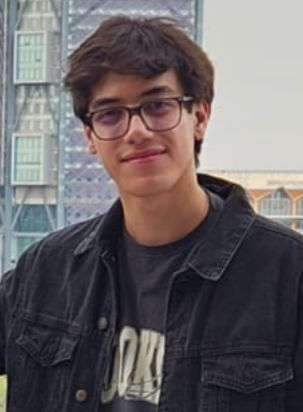
\includegraphics[height=3cm]{Medina.jpg} \\
				\textbf{Medina Alcazar,}\\ José Ángel \\ \texttt{l21330627@hermosillo.tecnm.mx} \\ Teléfono: 6623404696
			\end{tabular} &
			\begin{tabular}{c}
				
\includegraphics[height=3cm]{Soqui.jpg} \\
				\textbf{Vázquez Soqui,}\\ Diego Alberto \\ \texttt{l21330709@hermosillo.tecnm} \\ Teléfono: 6331076185
			\end{tabular}
		\end{tabular}
	\end{center}

\end{titlepage}

%	Es innecesario poner el índice porque ya aparece en los marcadores del PDF
%\tableofcontents
\tableofcontents
\pagebreak

% Ejemplo de inclusión de una sección (por ejemplo, "introduccion.tex" debe estar en la carpeta "secciones" y se recomienda no usar carácteres especiales (tilde) o espacios)
\section{\textbf{Introducción}}

El avance de la robótica ha sido posible en gran medida gracias a la integración de sensores que permiten a los robots percibir y responder a su entorno de manera eficiente. Los sensores son dispositivos esenciales que recopilan información sobre diversas variables y la convierten en señales procesables por el sistema de control del robot. Gracias a esta retroalimentación, los robots pueden mejorar su precisión, autonomía y capacidad de adaptación en diferentes entornos y tareas.

Los sensores utilizados en robótica pueden clasificarse en dos grandes categorías: sensores internos y sensores externos.

\subsection*{\quad\textbf{Sensores internos}}
Son aquellos que miden parámetros relacionados con el estado interno del robot, como la posición y velocidad de sus articulaciones, la aceleración, la fuerza aplicada por sus motores y el nivel de carga de su batería. Estos sensores son cruciales para garantizar el correcto funcionamiento del sistema mecánico y electrónico, evitando errores, optimizando el rendimiento y facilitando el mantenimiento preventivo. Algunos ejemplos incluyen encoders, giroscopios y sensores de corriente.

\subsection*{\quad\textbf{Sensores externos}}
Se encargan de captar información del entorno en el que opera el robot, permitiéndole interactuar con los objetos y adaptarse a diferentes condiciones. Estos sensores incluyen cámaras, sensores de proximidad, LIDAR, ultrasonidos y micrófonos, entre otros. Son fundamentales en aplicaciones como la navegación autónoma, la detección de obstáculos, el reconocimiento de patrones y la interacción con humanos.

\vspace{0.5cm}

El uso combinado de sensores internos y externos permite a los robots realizar tareas con un alto grado de precisión y eficiencia, ya sea en la automatización industrial, la robótica de servicio, la exploración espacial, la medicina o la robótica móvil. En este reporte, se analizarán en detalle los diferentes tipos de sensores empleados en robótica, su funcionamiento, sus aplicaciones y los desafíos asociados con su integración en sistemas autónomos.

A través de este estudio, se busca comprender la importancia de los sensores en la evolución de la robótica y cómo su desarrollo continúa impulsando la creación de robots cada vez más inteligentes, adaptables y funcionales en distintos campos de la tecnología.
\pagebreak
\section{\textbf{Sensores Internos}}
Los sensores internos se emplean para monitorear el estado interno de un robot, es decir, su posición, velocidad, aceleración, etc., en un momento determinado. Basado en estas informaciones, el controlador decide acerca del comando de control. Dependiendo de las diferentes cantidades que miden, los sensores se denominan como de posición, velocidad, aceleración o fuerza.

\subsection{\textbf{Sensores de Posición}}
Los sensores de posición miden la posición de cada articulación, es decir, el ángulo de articulación de un robot. A partir de dichos ángulos puede encontrarse la confi guración del ejecutor fi nal, y ubicar su posición y orientación por medio de la cinemática directa, que se revisará en el capítulo 6. A continuación se explican los diferentes sensores de posición.

\addcontentsline{toc}{subsubsection}{Encoder}
\subsection*{\quad\textbf{Encoder}}
El encoder es un dispositivo óptico digital que convierte el movimiento en una secuencia de pulsos digitales. Mediante el conteo de un solo bit o la decodificación de un conjunto de bits, los pulsos pueden convertirse en medidas relativas o absolutas. De este modo, los encoders son de tipo incremental o absoluto. Además, cada tipo puede ser lineal y rotatorio a su vez.

\begin{itemize}

	\item \textbf{Incremental}: este encoder tiene una escala transparente con una retícula opaca. El tamaño del espesor de las líneas de la retícula y el del espacio entre ellas son iguales y se encuentran en el rango de micrones. De un lado, la escala se equipa con una fuente de luz y un lente de condensador. Del otro, hay celdas sensibles a la luz. La resistencia de las celdas (fotodiodos) disminuye cada vez que reciben un rayo de luz. De este modo, se genera un pulso cada vez que un rayo de luz es atravesado por la línea opaca. Este pulso se introduce en el controlador que actualiza a un contador (un registro de la distancia recorrida).
	
	\item \textbf{Absoluto}: En principio, se parece al encoder lineal incremental. La diferencia es que da un valor absoluto de la distancia recorrida en cualquier momento. Así, las posibilidades de perder los pulsos a altas velocidades son menores. La salida es digital en este caso. La escala se marca con una secuencia de tiras opacas y transparentes. Si el bloque opaco que aparece en la escala de la ilustración representa 1 (uno) y el bloque transparente 0 (cero), entonces la columna de la extrema izquierda mostrará un número binario cómo 00000, es decir, un valor decimal de 0, y la columna siguiente mostrará un número binario 00001, es decir, una valor decimal de 1.
\end{itemize}

\begin{figure}[h] % h = aquí, t = top, b = bottom, p = página separada
	\centering
	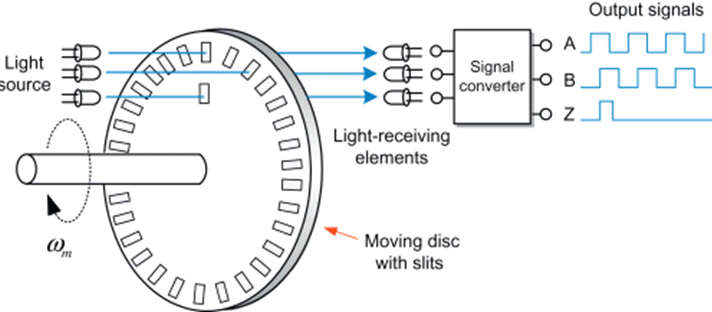
\includegraphics[width=0.6\textwidth]{encoderincr.jpg} % Ajusta el tamaño
	\caption{Encoder Incremental}
	\label{fig:ejemplo}
\end{figure}
\vspace{10cm}
\addcontentsline{toc}{subsubsection}{Potenciometro}
\subsection*{\quad\textbf{Potenciometro}}
Dispositivo de resistencia variable que expresa desplazamientos lineales o angulares en términos de voltaje, Consiste en una clavija deslizante que hace contacto con un elemento resistivo; conforme se mueve este punto de contacto, la resistencia entre el contacto deslizante y las conexiones de los extremos del dispositivo cambia en proporción al desplazamiento, x y  para potenciómetros lineales y angulares, respectivamente.

\addcontentsline{toc}{subsubsection}{LVDT}
\subsection*{\quad\textbf{LVDT}}
El transformador diferencial lineal variable (LVDT) es uno de los transductores de desplazamiento que más extensamente se usa, particularmente cuando se necesita alta precisión. Genera una señal de CA cuya magnitud se relaciona con el desplazamiento de un núcleo móvil. El concepto básico es el de un núcleo férrico que se mueve en un campo magnético, donde el campo se produce de un modo similar al campo de un transformador estándar. Existe un núcleo central, rodeado por dos bobinas secundarias idénticas y una bobina principal. Conforme el núcleo cambia su posición con respecto a las bobinas, cambia también el campo magnético y, por tanto, se modifica la amplitud de voltaje en la bobina secundaria como una función del desplazamiento del núcleo a través de un segmento considerable.

\addcontentsline{toc}{subsubsection}{Resólver}
\subsection*{\quad\textbf{Resólver}}
Los sincronizadores y resólvers son dispositivos analógicos que convierten la posición angular en señales eléctricas, a diferencia de los encoders digitales. Constan de un rotor giratorio y un estator estacionario, y requieren un convertidor analógico-digital para su procesamiento en computadoras. Los sincronizadores poseen tres devanados en el estator dispuestos a 120° en configuración "Y", lo que los hace más complejos y costosos, mientras que los resólvers tienen solo dos devanados a 90°, siendo más simples y económicos. Los resólvers modernos, especialmente los sin escobillas, utilizan un transformador para acoplar señales, eliminando el desgaste mecánico y aumentando su durabilidad. Operan en voltajes de 2V a 40V RMS y frecuencias de 400 Hz a 10 kHz, con precisiones angulares desde 5 hasta 0.5 minutos de arco. Su funcionamiento se basa en el principio del transformador rotatorio, donde la magnitud del voltaje inducido en el estator depende de la posición angular del rotor.


\subsection{\textbf{Sensores de Velocidad}}
Los sensores de velocidad realizan la medición tomando medidas de posición consecutivas a intervalos de tiempo constante, calculando la razón de cambio respecto al tiempo de los valores de posición, o lo determina en forma directa con base en diferentes principios.

\addcontentsline{toc}{subsubsection}{Todos los sensores de posición}
\subsection*{\quad\textbf{Todos los sensores de posición}}
Básicamente todos los sensores de posición, cuando se utilizan con ciertos límites de tiempo, pueden dar la velocidad, por ejemplo, el número de pulsos proporcionados por un encóder de posición incremental dividido entre el tiempo consumido en hacerlo. Sin embargo, este método impone una carga computacional sobre el controlador, que podrá estar ocupado por algunas otras operaciones.


\addcontentsline{toc}{subsubsection}{Tacómetro}
\subsection*{\quad\textbf{Tacómetro}}
Estos sensores pueden encontrar directamente la velocidad en cualquier momento y sin mucha carga computacional. Estos miden la velocidad de rotación de un elemento. Hay varios tipos de tacómetros en uso, pero un diseño sencillo se basa en la regla de Fleming, que declara que "el voltaje producido es proporcional al índice del acoplamiento inductivo". Aquí un conductor (básicamente una bobina) se sujeta al elemento rotativo que gira en un campo magnético (estator). Conforme incrementa la velocidad del eje, el voltaje producido en las terminales de las bobinas también aumenta. De otra manera, como se muestra en la figura 4.6, puede colocarse un imán sobre el eje rotativo y una bobina sobre el estator. El voltaje producido es proporcional a la velocidad de rotación del eje. Esta información se digitaliza mediante un convertidor analógico-digital y se introduce en la computadora.

\addcontentsline{toc}{subsubsection}{Sensor de Efecto Hall}
\subsection*{\quad\textbf{Sensor de Efecto Hall}}
Otro dispositivo de medición de velocidad es el sensor de efecto Hall, cuyo principio se describe a continuación. Si una pieza plana de material conductor llamada chip Hall se sujeta a una diferencia de potencial en sus dos lados opuestos, como se indica en la figura 4.7, entonces el voltaje que se genera a través de las caras perpendiculares es cero. Pero si un campo magnético se induce en ángulos rectos al conductor, el voltaje se genera en las otras dos caras perpendiculares. Entre más alto sea el valor de campo, más lo será el nivel de voltaje. Si se utiliza un imán anular, el voltaje producido será proporcional a la velocidad de rotación del imán.


\subsection{\textbf{Sensores de Aceleración}}
De manera parecida a las mediciones de velocidad que se dan a partir de la información de los sensores de posición, pueden encontrarse las aceleraciones como la razón de cambio respecto al tiempo de las velocidades obtenidas por los sensores de velocidad o calculado a partir de las informaciones de posición. Pero ésta no es una manera efi ciente para calcular
la aceleración, puesto que impondrá una carga de trabajo pesada sobre la computadora, lo que puede reducir la velocidad de operación del sistema. Otra forma de medir la aceleración es calculando la fuerza que resulta de multiplicar masa por aceleración.

\subsection{\textbf{Sensores de Fuerza}}
Una balanza de resorte es un ejemplo de un sensor de fuerza en donde se aplica una fuerza, por ejemplo, el peso, al platillo de balanza que causa un desplazamiento, es decir, el resorte se estira. El desplazamiento es entonces una medida de la fuerza. Existen otros tipos de sensores de fuerza, por ejemplo, con base en galgas, utilizando el sensor de efecto Hall, etcétera.

\addcontentsline{toc}{subsubsection}{Galgas Extensiométricas}
\subsection*{\quad\textbf{Galgas Extensiométricas}}
El principio de este sensor es que el alargamiento de un conductor aumenta su resistencia eléctrica. La resistencia eléctrica normal para galgas es de 50-100 ohmios. El incremento de resistencia se debe a: Incremento de la longitud del conductor; y Decremento en el área del conductor. Las deformaciones ocasionan cambios en la resistencia eléctrica de las galgas, lo que se mide mediante su conexión al circuito de puente de Wheatstone como una de las cuatro resistencias. Éste es un método barato y preciso para medir deformaciones.

\addcontentsline{toc}{subsubsection}{Sensor Piezoeléctrico}
\subsection*{\quad\textbf{Sensor Piezoeléctrico}}
Un material piezoeléctrico presenta un fenómeno conocido como efecto piezoeléctrico. Este efecto señala que cuando cristales elásticos asimétricos se deforman mediante una fuerza, se desarrollará un potencial eléctrico dentro de la red cristalina deformada. Este efecto es reversible. Esto quiere decir que si se aplica un voltaje entre las superficies del cristal, éste cambiará sus dimensiones físicas. La magnitud y polaridad de las cargas inducidas son proporcionales a la magnitud y dirección de la fuerza aplicada. Los materiales piezoeléctricos son cuarzo, turmalina, sal de Rochalle y otros. El rango de fuerzas que pueden medirse usando sensores piezoeléctricos es de 1 a 20 kN y con una proporción de 2×1052×105. Estos sensores pueden usarse para medir un cambio instantáneo en la fuerza (fuerzas dinámicas).
\cite{saha2014robotica}
\pagebreak






\section{Sensores Externos}
Los sensores externos se utilizan principalmente para saber más acerca del ambiente del robot, especialmente sobre los objetos que se va a manipular. Los sensores externos pueden
dividirse en las siguientes categorías:

\subsection{Tipo de Contacto}

\addcontentsline{toc}{subsubsection}{Interruptor de límite}
\subsection*{\quad\textbf{Interruptor de límite}}
El interruptor de límite tiene generalmente un brazo mecánico sensible a la presión. Cuando un objeto aplica presión sobre el brazo mecánico, se activa el interruptor. Es posible que un objeto tenga un imán que cause que un contacto suba y cierre cuando el objeto pase sobre el brazo. El registro de subida mantiene la señal en +V hasta que el interruptor cierra, transmitiendo la señal a tierra.\linebreak
Los interruptores de límite pueden ser normalmente abiertos (NO) o normalmente cerrados (NC) y pueden tener polos múltiples. Un interruptor normalmente abierto permite flujo de corriente hasta que se aplica presión al interruptor. 

\addcontentsline{toc}{subsubsection}{Interruptores Neumáticos}
\subsection*{\quad\textbf{Interruptores Neumáticos}}
Los sensores neumáticos se utilizan comúnmente para la detección de desplazamiento y proximidad sin contacto, utilizando para ello instalaciones de aire comprimido. Su funcionamiento se basa en que si el aire comprimido es expulsado y no se encuentra ningún impedimento en su liberación, en las proximidades de la salida del aire al exterior no se detectará ningún aumento de presión. Sin embargo, si el aire comprimido se encuentra con algún objeto en la proximidad del orificio de salida, se podrá detectar un aumento de presión. Este aumento de presión puede ser determinado y traducido en una medida de la distancia de proximidad del objeto que obstruye la salida del aire comprimido. Los sensores neumáticos no son sensibles a señales electromagnéticas lo que les hace robustos ante interferencias de ruidos externos de este tipo. Sin embargo, para su
funcionamiento se requiere la utilización de instalaciones de aire comprimido.

\addcontentsline{toc}{subsubsection}{Sensores Piezoeléctricos}
\subsection*{\quad\textbf{Sensores Piezoeléctricos}}
Los sensores piezoeléctricos están constituidos por materiales o cristales iónicos que generan una pequeña cantidad de energía eléctrica cuando son deformados. Estos sensores son utilizados para mediciones de fuerzas y presiones aplicadas con un corto periodo de tiempo.
Cuando sobre materiales piezoeléctricos como el titanato de bario se le aplica una fuerza, las cargas negativas del material se concentran en un lado mientras que el opuesto queda cargado positivamente, generando consecuentemente un voltaje (también se producirá un cambio en Ia capacitancia).

\addcontentsline{toc}{subsubsection}{Transductores de Presión}
\subsection*{\quad\textbf{Transductores de Presión}}
Un transductor de presión, a veces llamado transmisor de presión, es un transductor que convierte presión en una señal eléctrica analógica. Aunque hay varios tipos de transductores de presión, uno de los más comunes es el transductor de base de calibrador de tensión. La conversión de presión en una señal eléctrica se logra mediante la deformación física de medidores de tensión que están unidos al diafragma del transductor de presión y cableados a una configuración de puente de Wheatstone. La presión aplicada al transductor de presión produce una deflexión del diafragma que introduce tensión en los calibradores. La tensión producirá un cambio en la resistencia eléctrica proporcional a la presión. \cite{OmegaPressureTransducers}

\subsection{Tipo Sin Contacto}

\addcontentsline{toc}{subsubsection}{Sensor de Proximidad}
\subsection*{\quad\textbf{Sensor de Proximidad}}
La detección de proximidad es la técnica que se usa para detectar la presencia o ausencia de un objeto por medio de un sensor electrónico sin contacto. Hay dos tipos de sensores de proximidad: inductivo y capacitivo. Los sensores de proximidad inductivos se usan en lugar de interruptores de límite para la detección sin contacto de objetos metálicos. Los sensores de proximidad capacitivos se usan sobre la misma base que los sensores de proximidad inductivos, pero también pueden detectar objetos no metálicos.



\pagebreak

\section{Imágenes}
En \LaTeX, las imágenes se pueden incluir utilizando el paquete \texttt{graphicx}. 
Para añadir una imagen en texstudio, es posible arrastrarla directamente en el editor, lo que obtendrá como resultado lo mostrado en la \autoref{fig:insertarimagen}.

\begin{figure}[h]
	\centering
	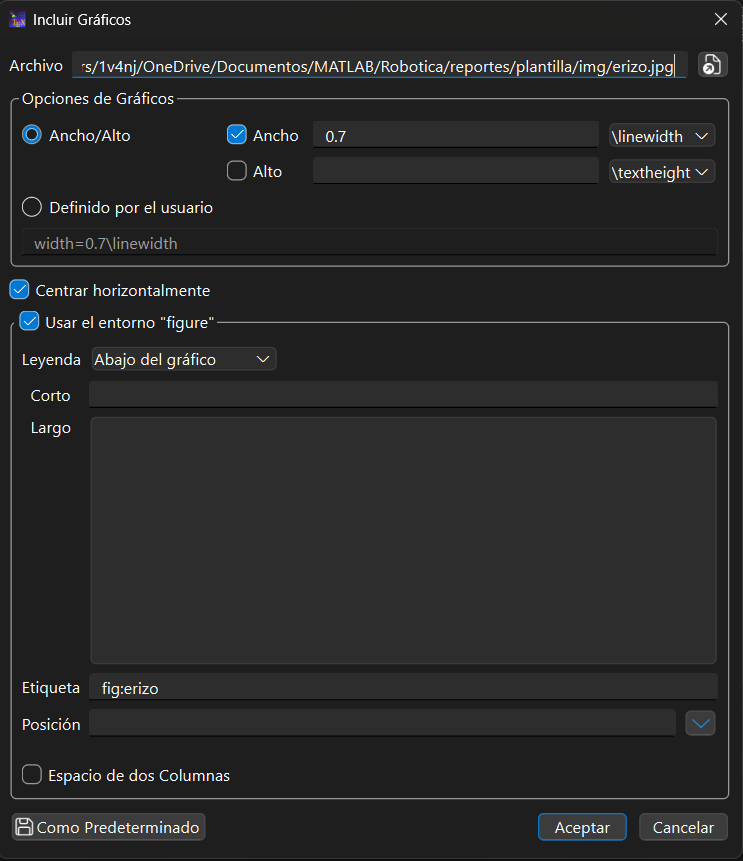
\includegraphics[width=0.7\linewidth]{img/insertarImagen}
	\caption{Opciones al insertar una imagen}
	\label{fig:insertarimagen}
\end{figure}

Algunas opciones clave incluyen:

\begin{itemize}
	\item \textbf{Tamaño de la imagen}: Se puede definir un ancho o alto relativo a la caja de texto o se puede usar un tamaño en pixeles (px), centímetros (cm) o el ancho de la letra M (em).
	\item \textbf{Centrado}: Se puede marcar la opción para que la imagen aparezca centrada automáticamente.
	\item \textbf{Uso del entorno `figure'}: Permite que la imagen tenga una numeración automática y pueda referenciarse en el texto con \texttt{\textbackslash ref\{\}} o \texttt{\textbackslash autoref\{\}}.
	\item \textbf{Posicionamiento (`h`, `t`, `b`, `p`)}: Al presionar la flecha de la derecha, podemos añadir las opciones que determinan la posición de la imagen en el documento, como después del texto o arriba de la página, etc. Si igual vamos a referenciar las figuras, es innecesario que estén exactamente donde fueron mencionadas ya que eso deja muchos espacios en blanco.
	\item \textbf{Leyenda Largo}: permite poner una descripción de la imagen en el lugar que elegimos (debería de estar debajo).
	\item \textbf{Etiqueta}: nos servirá para referenciarla. 
\end{itemize}

Para usar dos imágenes como en \autoref{fig:mascotas}, se utilizó \texttt{subfloat}.
% Dos imágenes de mascotas
\begin{figure}[h]
	\centering
	\subfloat[Perro]{%
		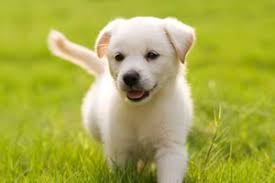
\includegraphics[width=0.4\textwidth]{perro.jpg}%
		\label{fig:perro}
	}
	\hfill
	\subfloat[Gato]{%
		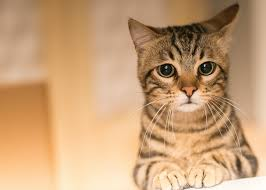
\includegraphics[width=0.4\textwidth]{gato.jpg}%
		\label{fig:gato}
	}
	\caption{Imagen de dos mascotas}
	\label{fig:mascotas}
\end{figure}
\section{Tablas}
Existen varias formas de crear tablas además de este entorno, como \texttt{array}, \texttt{longtable} y \texttt{tabularx}, que permiten manejar datos extensos de manera eficiente. También es posible convertirlas desde páginas, como en \href{https://tableconvert.com/es/excel-to-latex}{TableConvert}, que permite transformar datos de Excel a formato \LaTeX fácilmente.

A continuación, se presenta una tabla larga como ejemplo:

\newcounter{actividad} % Define un contador llamado "actividad"
\begin{longtable}{|c|p{10cm}|c|} % Define anchos específicos
	\caption{Ejemplo de Tabla Larga.} \label{tab:ejemplo_tabla} \\
	\hline
	\textbf{No.} & \textbf{Descripción} & \textbf{Estado} \\
	\hline
	\endfirsthead
	\multicolumn{3}{c}{{\tablename\ \thetable{} -- continuación}} \\
	\hline
	\textbf{No.} & \textbf{Descripción} & \textbf{Estado} \\
	\hline
	\endhead
	\hline \multicolumn{3}{r}{{Continúa en la siguiente página...}} \\
	\hline
	\endfoot
	\hline
	\endlastfoot
	% Contenido de la tabla
	1 & Lorem ipsum dolor sit amet, consectetur adipiscing elit. & Completado \\
	2 & Sed do eiusmod tempor incididunt ut labore et dolore magna aliqua. & En proceso \\
	3 & Ut enim ad minim veniam, quis nostrud exercitation ullamco laboris. & Pendiente \\
	4 & Duis aute irure dolor in reprehenderit in voluptate velit. & Pendiente \\
	5 & Excepteur sint occaecat cupidatat non proident. & Pendiente \\
	6 & Sunt in culpa qui officia deserunt mollit anim id est laborum. & Pendiente \\
	7 & Curabitur pretium tincidunt lacus, nulla gravida orci a odio. & Pendiente \\
	8 & Nullam varius, turpis et commodo pharetra. & Pendiente \\
	9 & Sed ac orci quis tortor imperdiet venenatis. & Pendiente \\
	10 & Duis eget orci sit amet orci dignissim rutrum. & Pendiente \\
	11 & Nam dui ligula, fringilla a, euismod sodales, sollicitudin vel, wisi. & Pendiente \\
	12 & Pellentesque habitant morbi tristique senectus et netus et malesuada. & Pendiente \\
	13 & Fusce convallis metus id felis luctus adipiscing. & Pendiente \\
	14 & Pellentesque dapibus hendrerit tortor. & Pendiente \\
	15 & Praesent egestas tristique nibh. & Pendiente \\
	16 & Curabitur a felis in nunc fringilla tristique. & Pendiente \\
	17 & Phasellus nec sem in justo pellentesque facilisis. & Pendiente \\
	18 & Etiam imperdiet imperdiet orci. & Pendiente \\
	19 & Vestibulum ante ipsum primis in faucibus orci luctus et ultrices. & Pendiente \\
	20 & Quisque id mi. Integer ante arcu, accumsan a, consectetuer eget, posuere ut, mauris. & Pendiente \\
\end{longtable}
\section{Ecuaciones}
Para realizar ecuaciones, se pueden ayudar mucho de ChatGPT (Como copiar una imagen y que lea la ecuación para dártela en formato \LaTeX) y de que MATLAB, word y algunas páginas te permiten copiar ecuaciones en formato \LaTeX. El modelo en espacio de estados de un robot de dos grados de libertad, el cual se puede ver en el Capítulo 5: Dinámica del Robot en \cite{barrientos2007fundamentos} se expresa como

\begin{equation}
	\label{eq:spaceStateRobot}
	\begin{bmatrix}
		\dot{q} \\
		\ddot{q}
	\end{bmatrix} =
	\begin{bmatrix}
		0 & I \\
		M^{-1}(-C - G)
	\end{bmatrix}
	\begin{bmatrix}
		q \\
		\dot{q}
	\end{bmatrix} +
	\begin{bmatrix}
		0 \\
		M^{-1} B
	\end{bmatrix} u,
\end{equation}
donde:
\begin{itemize}
	\item \( q \) es el vector de posiciones articulares del robot.
	\item \( \dot{q} \) y \( \ddot{q} \) son las velocidades y aceleraciones articulares.
	\item \( M \) es la matriz de inercia.
	\item \( C \) representa las fuerzas centrífugas y de Coriolis.
	\item \( G \) es el vector de fuerzas gravitacionales.
	\item \( B \) es la matriz de entrada de los torques.
	\item \( u \) es el vector de torques aplicados a las articulaciones.
\end{itemize}

Cabe destacar que en \eqref{eq:spaceStateRobot}, la ecuación se referencia después de haberla nombrado y forma parte de la oración, por lo que debe llevar puntos o comas. También al referenciar, debe de estar entre paréntesis con \texttt{eqref}.
\section{Conclusión} \label{sec:conclusion}
Solo añadan esta sección si lo consideran necesario. No es deben poner un resumen del contenido ni información importante que no se haya mencionado en una sección principal. Pueden poner la parte en la que más batallaron, el conocimiento más importante que consideran haber obtenido o algún comentario.
\subsection{Persona 1}
En caso de que haya sido una perspectiva individual, tienen que poner los comentarios de cada integrante y su nombre.
\subsection{Persona 2}
Esto me dará una retroalimentación desde la perspectiva de diferentes alumnos con diferentes roles.
\pagebreak

%-------------------------------------------
% Bibliografía
%-------------------------------------------
\bibliographystyle{IEEEtran}  % Estilo de bibliografía IEEE
% La bibliografía se tomará del archivo "fuentes.bib"
\bibliography{fuentes}
	
\end{document}
